\documentclass[fleqn,11pt]{article}
\usepackage[letterpaper,margin=1in]{geometry}
\usepackage{amsmath}
\usepackage{tikz}
\usepackage{booktabs}
\usepackage{graphicx}
\usepackage{listings}
\usepackage{minted}
\usepackage{titling}
\usepackage{xcolor}
\usepackage{siunitx}

\sisetup{detect-weight=true, binary-units=true}
\usetikzlibrary{arrows,automata,positioning}

\makeatletter
\def\@maketitle{   % custom maketitle 
	{\Large \bfseries \@title}
	\hfill \theauthor
	\smallskip \hrule \bigskip }
%\renewcommand{\section}{\@startsection
%   	{section}%                   % the name
%   	{1}%                         % the level
%   	{0mm}%                       % the indent
%   	{.8\baselineskip}%            % the before skip
%   	{0.1\baselineskip}%          % the after skip
%   	{\bfseries}} % the style
\makeatother
\setlength{\parindent}{1.4em}
\setminted{
framesep=2mm,
baselinestretch=1.2,
fontsize=\footnotesize,
linenos
}

\title{CS 460: Networking Simulation}
\author{Kevin Haroldsen}
\date{}


\begin{document}

\maketitle

\section{Summary}
In this report, I give the results of running different programs using the \texttt{bene} simulator.
The first, with two nodes, highlights the difference in timing for propagation and transmission delay.
The second, with three nodes, highlights how queuing delay works together with transmission and propagation delays.
The last uses two nodes and exponential delay to highlight how fractional load on a network interacts with queuing delay.

I managed to have some difficulty in getting the simulator to work as I wanted to.
A bidirectional two-node link was simple to set up,
but getting a unidirectional three-node link to forward properly to the third node was much more difficult than expected.

I made many quality of life improvements to the library, including some static typing.
The semantics of forwarding was also modified to allow for more logical usage.
I also made a very useful \texttt{NetHelper} class, which managed many of the more complicated simulation operations, such as sending packets to other nodes or creating forwarding entries.

\section{Two Nodes}
Calculating the theoretical arrival time would be
$ \frac{8L}{R} + p $,
where $ L $ is the length of the message in bytes,
$ R $ is the bandwidth of the link in bits/second,
and $ p $ is the propagation delay of the link.

\newcommand{\twonodes}[2]{%
\begin{tikzpicture}[on grid,auto,node distance=3cm,baseline]%
\node[state] (n1) {$ n_1 $};%
\node[state] (n2) [right of=n1] {$ n_2 $};%
\path[<->] (n1) edge node [above] {#1} node [below] {#2} (n2);%
\end{tikzpicture}%
\vspace{.5em}
}

\begin{enumerate}
\itemsep2em
\item
\textbf{Network Configuration:}

\twonodes{1 Mbps}{1 sec}

\textbf{Output:}
\begin{minted}[linenos=]{text}
0.000 0 1.008
\end{minted}

\textbf{Calculation:}
\[
\dfrac{8L}{R} + p =
\dfrac{\SI{8000}{\bit}}{\SI{1}{\mega\bit\per\sec}} + \SI{1}{\sec} =
\SI{1.008}{\sec}
\]

Clearly, the propagation delay is the primary cause of the delay in this scenario.

\item
\textbf{Network Configuration:}

\twonodes{100 bps}{10 ms}

\textbf{Output:}
\begin{minted}[linenos=]{text}
0.000 0 80.010
\end{minted}

\textbf{Calculation:}
\[
\dfrac{8L}{R} + p =
\dfrac{\SI{8000}{\bit}}{\SI{100}{\bit\per\sec}} + \SI{10}{\ms} =
\SI{80.010}{\sec}
\]

In this case, 80 seconds of delay is caused by the abysmally slow bandwidth.

\item
\textbf{Network Configuration:}

\twonodes{1 Mbps}{10 ms}

\textbf{Output:}
\begin{minted}[linenos=]{text}
0.000 0 0.018
0.000 1 0.026
0.000 2 0.034
2.000 3 2.018
\end{minted}

\textbf{Calculation:}

For the first packet:
\[
\dfrac{8L}{R} + p =
\dfrac{\SI{8000}{\bit}}{\SI{1}{\mega\bit\per\sec}} + \SI{10}{\ms} =
\SI{18}{\ms}
\].

After that, the next two packets simply add the transmission delay (\SI{8}{\ms}).
Then, the fourth packet, delayed after 2 seconds, will have the same \SI{18}{\ms} to reach the end as the first packet.

\end{enumerate}

\section{Three Nodes}
For three nodes, I define the transmission delays $ t_1 = \frac{8L}{R_1} $ and $ t_2 = \frac{8L}{R_2} $, and the propagation delays $ p_1 $ and $ p_2 $, and $ p = p_1 + p_2 $.
Assuming that packets are sent one after another, and $ t_1 \leq t_2 $,
packet $ n $ will arrive at the third node after
$ t_1 + n t_2 + p $.

\begin{enumerate}

\newcommand{\threenodes}[4]{%
    \begin{tikzpicture}[on grid,auto,node distance=3cm,baseline]%
    \node[state] (n1) {$ n_1 $};%
    \node[state] (n2) [right of=n1] {$ n_2 $};%
    \node[state] (n3) [right of=n2] {$ n_3 $};%
    \path[->] (n1) edge node [above] {#1} node [below] {#2} (n2);%
    \path[->] (n2) edge node [above] {#3} node [below] {#4} (n3);%
    \end{tikzpicture}%
    \vspace{.5em}
}

\item \textbf{Two Fast Links}

\textbf{Network Configuration:}

\threenodes{1 Mbps}{100 ms}{1 Mbps}{100 ms}

\textbf{Output:}
\begin{minted}[linenos=]{text}
7.960 995 8.176
7.968 996 8.184
7.976 997 8.192
7.984 998 8.200
7.992 999 8.208
\end{minted}

\textbf{Calculation:}
\[
t_1 + n t_2 + p =
\dfrac{\SI{8000}{\bit}}{\SI{1}{\mega\bit\per\sec}} +
1000 \dfrac{\SI{8000}{\bit}}{\SI{1}{\mega\bit\per\sec}} +
\SI{200}{\ms} =
\SI{8.208}{\sec}
\]


For a single packet, the propagation delay dominates.
However, over the entire file, the transmission delay of 8 seconds is the largest factor.

\item \textbf{One Fast Link, One Slow Link}

\textbf{Network Configuration:}

\threenodes{1 Mbps}{100 ms}{256 Kbps}{100 ms}

\textbf{Output:}
\begin{minted}[linenos=]{text}
7.960 995 31.333
7.968 996 31.364
7.976 997 31.396
7.984 998 31.427
7.992 999 31.458
\end{minted}

\textbf{Calculation:}
\[
t_1 + n t_2 + p =
\dfrac{\SI{8000}{\bit}}{\SI{1}{\mega\bit\per\sec}} +
1000 \dfrac{\SI{8000}{\bit}}{\SI{256}{\kilo\bit\per\sec}} +
\SI{200}{\ms} =
\SI{31.458}{\sec}
\]

For a single packet, the propagation delay dominates.
Over the entire file, the majority of time the packets wait is in the queue of $ n_2 $.

\end{enumerate}

\section{Queuing Theory}
\textbf{Network Configuration:}

\twonodes{1 Kbps}{1 ms}

\noindent
\textbf{Load Settings:}

I simulated continually sending 1000-byte packets at varying loads, for 100,000 seconds.
For each of these, I outputted the queuing delay and link load of each item into a CSV file.

\noindent
\textbf{Results:}
\begin{center}
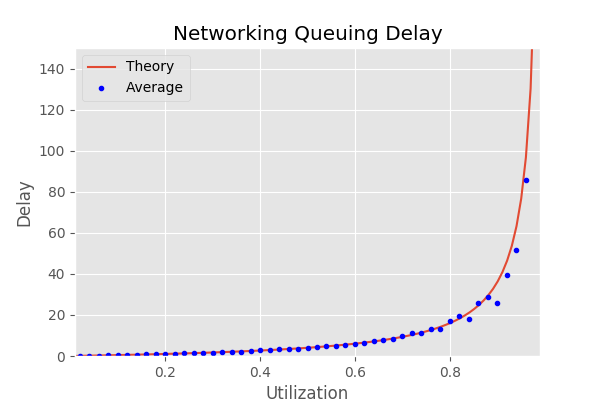
\includegraphics{graphs/queueing}
\end{center}

I used \texttt{pandas} to load the data points, average the queuing delay for each utilization, and plot it.
Along with the results, I also plotted the theoretical queuing delay:
\[
\frac{1}{2 \mu} \cdot \frac{\rho}{1-\rho}
\]

The similarity indicates that the simulator is working as intended.

\section{Conclusion}
In conclusion, the simulator does work, even if some finagling had to be done to get it to work as I had expected.
The theoretical results and simulated results match very closely.

I already had experience with Python, \texttt{matplotlib}, and \LaTeX.
I spent more time than expected investigating how routing is supposed to work between nodes.
I made modifications to make it so that an address of a destination node is the address of a link where it is an endpoint.
This made automatic route calculation much simpler, and now for future simulations, usage of the library is much more succinct.

Overall, this was an interesting lab, and I learned quite a bit, including using \texttt{pandas}. 
I also had to think quite a bit on how to calculate three-node delays with different link speeds.
I'm looking forward to working on the next lab.

\end{document}
